

\documentclass[twoside,twocolumn]{article}

\usepackage{blindtext} % Package to generate dummy text throughout this template 
\usepackage{graphicx}
\usepackage[sc]{mathpazo} % Use the Palatino font
\usepackage[T1]{fontenc} % Use 8-bit encoding that has 256 glyphs
\linespread{1.05} % Line spacing - Palatino needs more space between lines
\usepackage{microtype} % Slightly tweak font spacing for aesthetics

\usepackage[english]{babel} % Language hyphenation and typographical rules

\usepackage[hmarginratio=1:1,top=32mm,columnsep=20pt]{geometry} % Document margins
\usepackage[hang, small,labelfont=bf,up,textfont=it,up]{caption} % Custom captions under/above floats in tables or figures
\usepackage{booktabs} % Horizontal rules in tables

\usepackage{lettrine} % The lettrine is the first enlarged letter at the beginning of the text

\usepackage{enumitem} % Customized lists
\setlist[itemize]{noitemsep} % Make itemize lists more compact

\usepackage{abstract} % Allows abstract customization
\renewcommand{\abstractnamefont}{\normalfont\bfseries} % Set the "Abstract" text to bold
\renewcommand{\abstracttextfont}{\normalfont\small\itshape} % Set the abstract itself to small italic text

\usepackage{titlesec} % Allows customization of titles
\renewcommand\thesection{\Roman{section}} % Roman numerals for the sections
\renewcommand\thesubsection{\roman{subsection}} % roman numerals for subsections
\titleformat{\section}[block]{\large\scshape\centering}{\thesection.}{1em}{} % Change the look of the section titles
\titleformat{\subsection}[block]{\large}{\thesubsection.}{1em}{} % Change the look of the section titles

\usepackage{fancyhdr} % Headers and footers
\pagestyle{fancy} % All pages have headers and footers
\fancyhead{} % Blank out the default header
\fancyfoot{} % Blank out the default footer
\fancyhead[C]{Titulo $\bullet$ Junio 2019 $\bullet$ } % Custom header text
\fancyfoot[RO,LE]{\thepage} % Custom footer text

\usepackage{titling} % Customizing the title section

\usepackage{hyperref} % For hyperlinks in the PDF

%----------------------------------------------------------------------------------------
%	TITLE SECTION
%----------------------------------------------------------------------------------------

\setlength{\droptitle}{-4\baselineskip} % Move the title up

\pretitle{\begin{center}\Huge\bfseries} % Article title formatting
\posttitle{\end{center}} % Article title closing formatting
\title{Virtualizacion y Contenedores} % Article title
\author{Andre Reinoso, Samuel Nuñez, Andres De la Barra ,David Damian y Richard Cruz}
\date{\today} % Leave empty to omit a date
\renewcommand{\maketitlehookd}{%
\begin{abstract}
\noindent Ingles
\end{abstract}
\begin{abstract}
\noindent Español.
\end{abstract}
}

%----------------------------------------------------------------------------------------

\begin{document}

% Print the title
\maketitle

%----------------------------------------------------------------------------------------
%	ARTICLE CONTENTS
%----------------------------------------------------------------------------------------

\section{Introduccion}

\lettrine[nindent=0em,lines=3]{L}a virtualiza



%------------------------------------------------

\section{Objetivos}

\begin{itemize}
\item Entender qué es una máquina virtual.
\item Entender qué es un contenedor.
\item Comparar ambos conceptos.
\item Establecer un juicio acerca de las ofertas y el potencial de ambas.

\end{itemize}




%------------------------------------------------

\section{Desarrollo}

\subsection{¿Que es una maquina virtual?}

Una máquina virtual 

\begin{center}
	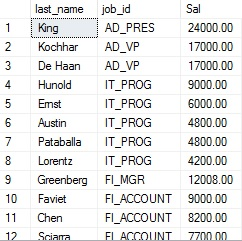
\includegraphics[width=5cm]{./Imagenes/virtualizacion} 
	\end{center}




\subsection{Grafos}

Las bases de datos NoSQL en grafo permiten representar los datos utilizando estructuras de grafos. Un grafo es una representación abstracta de un conjunto de objetos. Los objetos de los grafos se representan mediante vértices (también llamados nodos) y aristas.

\begin{center}
	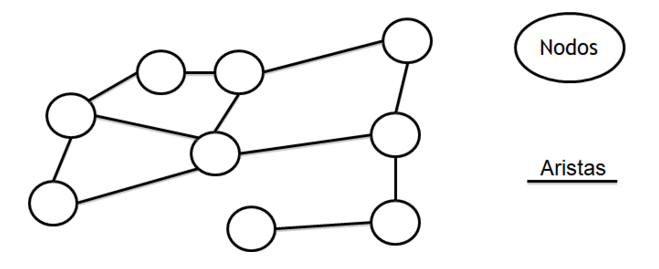
\includegraphics[width=7cm]{./Imagenes/nodos_aristas} 
\end{center}

El modelo en grafo es útil cuando los datos a almacenar tienen multitud de interrelaciones entre sí, y cuando la importancia recae más en las interrelaciones que se establecen entre los datos, que en los propios datos en sí. 
\\
En consecuencia, este tipo de bases de datos tiende a almacenar pocos datos de los objetos del mundo real que se desean representar pero muchos datos sobre sus interrelaciones, a diferencia de lo que acostumbra a suceder en las bases de datos relacionales, donde hay muchos datos de los objetos (representados mayoritariamente en las propiedades o atributos de las relaciones) y pocas interrelaciones entre los objetos (representadas mediante claves foráneas). 


\begin{itemize}
\item Ejemplo
\\ A continuación podemos ver un ejemplo simple en el que hemos creado un grafo con dos tweets (en color verde) y dos usuarios de Twitter (en color azul). Como vemos, los tweets y los usuarios se han etiquetado con las etiquetas “Tweet” y “TwitterUser” para indicar su tipo. Vemos también que uno de los tweets es un reply (se indica mediante una relación con una etiqueta “Reply”) y que los dos usuarios de Twitter se siguen mútuamente (se indica mediante la etiqueta “Follows”). También se indican los autores de cada tweet (mediante la etiqueta “Author”).


\begin{center}
	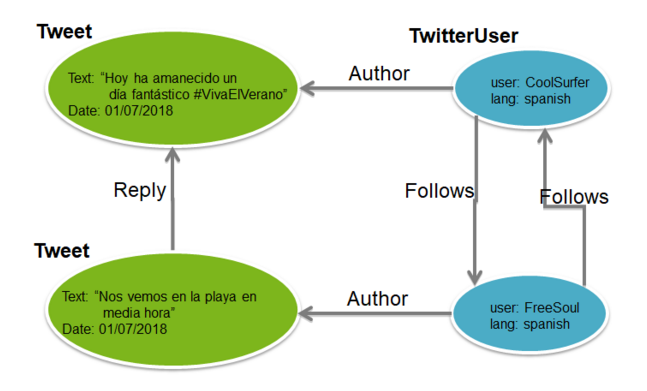
\includegraphics[width=7cm]{./Imagenes/tweet} 
\end{center}

\end{itemize} 

\subsection{Tabular Column-Store}
El objetivo pri

\begin{itemize}
	\item Jerarquia maquina virtual
	\\La primer gran diferencia es la jerarquia, forma de como estan constituidas. En el primero de los casos las maquinas virtuales estan constituidas por:

	\begin{center}
	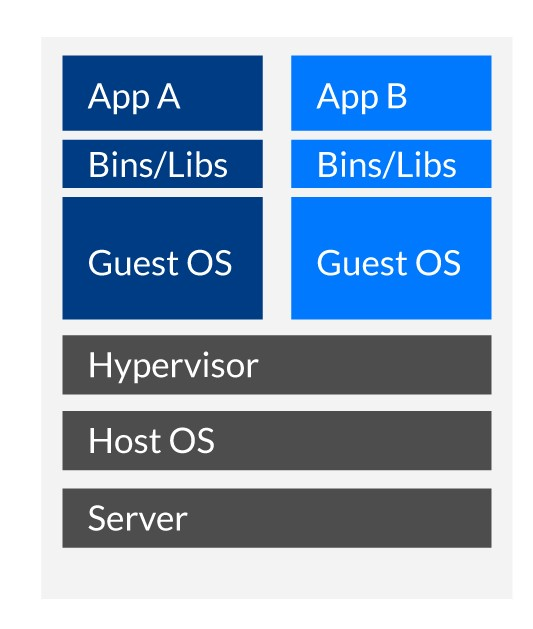
\includegraphics[width=5cm]{./Imagenes/jerarquia1} 
	\end{center}
\end{itemize} 

\begin{itemize}
	\item Jerarquia contenedor
	\\ \textbf{-El servidor o una computador}.

	\begin{center}
	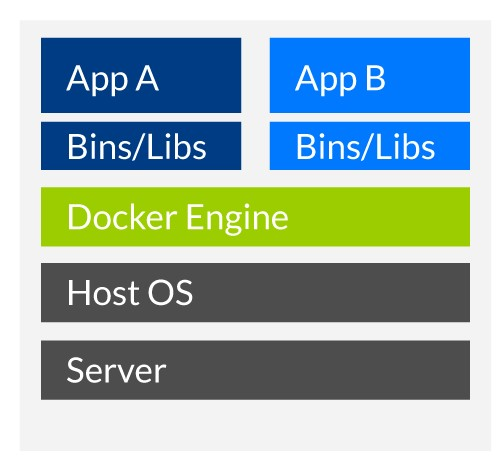
\includegraphics[width=5cm]{./Imagenes/jerarquia2} 
	\end{center}
\end{itemize} 

\begin{itemize}
	\item Los contenedores permiten desplegar aplicaciones más rápido, arrancarlas y pararlas más rápido y aprovechar mejor los recursos de hardware.




\end{itemize} 

\section{Conclusiones}

Para hablar de contenedores y
%	REFERENCE LIST
%----------------------------------------------------------------------------------------

\begin{thebibliography}{99} % Bibliography - this is intentionally simple in this template

\bibitem[Martin, 2011]{Diego Martin:2011dg}
Martin, M.M,  y J.U (2011).
\newblock Virtualización, una solución para la eficiencia,
seguridad y administración de intranets
\newblock {\em El profesional de la informacion}, 350.
\newblock Contenedor de aplicaciones: Docker (2015)
 
 
\end{thebibliography}

%----------------------------------------------------------------------------------------

\end{document}
